\documentclass[a4paper,11pt]{jsbook}

\newcommand{\V}[1]{\boldsymbol{#1}}
\def\thline{\noalign{\hrule height 1pt}}
\def\tvline{\vrule width 1pt}

\usepackage{here} %図の場所の指定で[H](ここに貼る)を指定するためのパッケージ
\usepackage{makeidx}
\usepackage{amsmath}
\usepackage{amssymb}
\usepackage[dvipdfmx]{graphicx} %dvipdfmxはjpgやpngの張り込みのために使用
\usepackage{algorithmic}
\usepackage{algorithm}
\usepackage{subcaption}
\usepackage{url}
% \makeindex

\pagenumbering{roman}

\begin{document}
% 表紙
\title{令和3年度 卒業論文\\
各パーティクルごとに観測範囲を付与した\\モンテカルロ自己位置推定}

\author{池邉 龍宏 \\
Chiba Institute of Technology}

\date{2022年2月15日}

\maketitle

\chapter*{謝辞}\addcontentsline{toc}{chapter}{謝辞}

本稿を執筆するにあたって助言を頂いた上田隆一准教授および
上田研究室のみなさまに感謝します。



\tableofcontents

%\cleardoublepage

%%% 本文 %%%
% 章のページの先頭は左側(奇数ページ)に来る

\cleardoublepage
\pagenumbering{arabic}
 
\chapter{序論}

\section{研究背景}

安定的に自己位置推定を行うことは, 移動ロボット
が, ある目標地点へと自律移動を行うために重要である. 
移動ロボットが自己位置を推定する方法として,
確率的な位置推定法である, パーティクルフィルタ
がよく用いられる. 
%@@@rosは大文字じゃないですかね!!
用いられている例として, ROSのナビゲーションスタックである
amcl\cite{amcl_github}や千葉工業大学未来ロボティクス学科の上田隆一准教授が
開発したemcl\cite{emcl_github}がある. 
パーティクルフィルタは現在の状態から推定される次のロボットの状態の候補として
多数のパーティクルで近似し, 予測と観測によって,
パーティクルの姿勢を更新することで自己位置を推定するアルゴリズムである.
%@@@置き換え????
%@@@パーティクルの何を更新すんの?
しかし, パーティクルフィルターにおいて何らかの理由で
ロボット位置の真値と全パーティクルの位置における整合性が低い場合, 
%@@@「尤もらしさ」って説明してない言葉を使わない. 
自己位置推定を誤ってしまう. 
(以後, ロボット位置の真値と全パーティクルの位置における整合性については尤度および尤もらしさと表現する. )
自己位置推定を誤ったまま行動をし続けてしまった場合, 
ロボットが走行できない状態になってしまう. 
そのような例として, 以下のような例がある. 

\begin{itemize}
  \item 観測できない低い障害物と衝突し, スタック
  \item 経路計画が不安定になり, スタック
  \item 誘拐問題\cite{gutmann2002etal}に発展し, スタック
\end{itemize}
%@@@スタックという言葉をここで説明. 

\noindent
スタックとは, ロボットが走行不能な状態に陥ってしまうことである. 

自己位置推定を誤ってしまう原因として未知障害物の観測がある. 
未知障害物は図\ref{fig:unknown-obstacles}, \ref{fig:known-obstacles}
に見られる既知のマップに含まれていない観測情報のことである. 
%@@@「のような」->「に見られる」
例えば, 既知のマップに対して未知障害物である車や人を含んだ観測情報
をパーティクルの尤度計算に用いた場合, 全パーティクルの尤もらしさが低下する. 
また, 未知障害物への対策を講じていなければ, 未知障害物が観測情報に含まれている間は
常に全パーティクルの尤もらしさが低下し続け, パーティクルの分布は大きく広がってしまい, 
自己位置推定が破綻してしまう. また, 自己位置推定を誤ってしまった状態に対しての回復策として
様々なリセット法がある. 
例えば, amclは前回より尤度平均が小さくなるとランダムパーティクルを注入する. 
emclは尤度平均がある任意の閾値より小さくなった場合, 
任意の範囲内にパーティクルを配置をする\cite{ueda2004iros}. 
それぞれのリセットはいずれも尤度がある値を下回った時にかかり, 
パーティクルの分布を真値周辺に近づけることができる. 
しかし, 効果的なリセットではあるが未知障害物を観測した場合, 
不要なリセットが何度もかかってしまうことで, かえって自己位置推定に悪影響を与える
ことがある. 
このような場合, 全てのパーティクルにおいて, 何らかの方法により
未知障害物を含まない同じ観測情報を使用するような, 
未知障害物を含んだ観測情報を尤度計算に使用しないことによる解決方法が考えられる. 
そのため, 本稿ではパーティクルが未知障害物を含まない観測情報を使用する方法について着目した. 

\begin{figure}[htbp]
  \begin{minipage}[b]{0.5\linewidth}
    \centering
    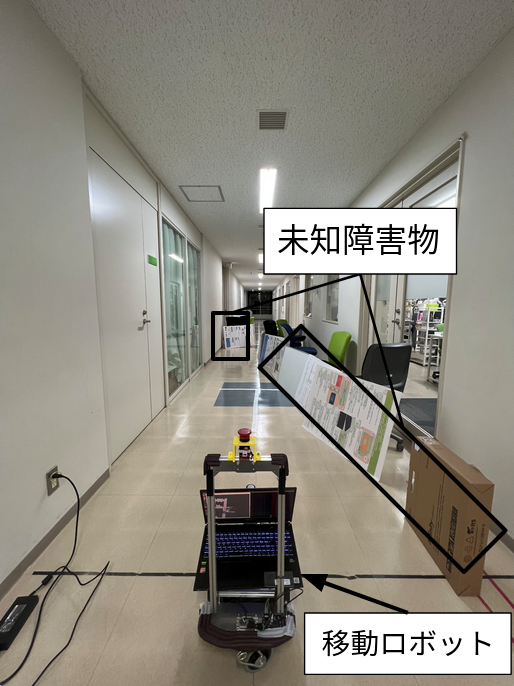
\includegraphics[keepaspectratio, scale=0.32]{figs/unknown_obstacles.png}
    \caption{未知障害物を含んだ屋内環境}
    \label{fig:unknown-obstacles}
  \end{minipage}
  \begin{minipage}[b]{0.5\linewidth}
    \centering
    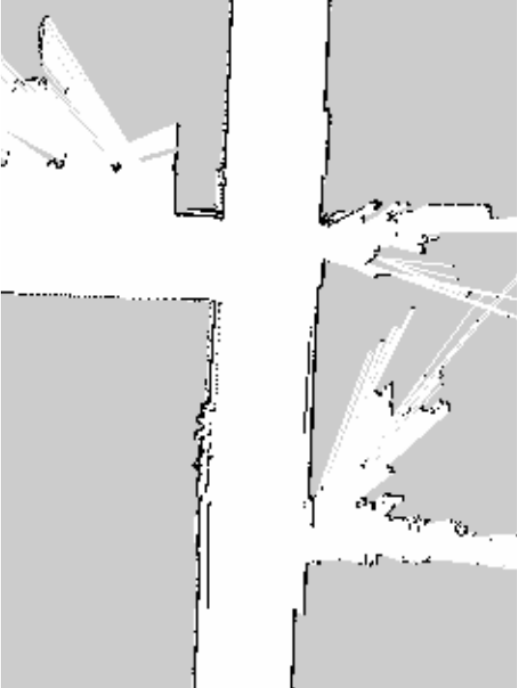
\includegraphics[keepaspectratio, scale=0.32]{figs/known_obstacles.png}
    \caption{未知障害物を含んでいない地図}
    \label{fig:known-obstacles}
  \end{minipage}
\end{figure}

%%%%ここで段落は分ける. というか, 1.2: 従来研究に移行しましょう. これ以降はまた次の機会に見ます. 
%%%%掛かる<-漢字の間違い

\section{従来研究}

安定的に自己位置推定を行うためには未知障害物に対応するアルゴリズムが必要である.
そのため, 自己位置推定において未知障害物に対応するための研究事例\cite{富沢2012}\cite{赤井2019}がある. 
\cite{富沢2012}はセンサの観測情報から得られたローカル地図と既知の地図
とで重なり合ったピクセルごとの差異を求め不一致のピクセル数から
そのパーティクルの尤もらしさを判定する方法による未知障害物の対策を提案している. 
この方法の場合, 使用するセンサの計測距離に応じてマッチングに使用するための地図が大きくなり, 
ピクセルごとの差異を求める際の計算コストの増加が考えられる. 
また, \cite{赤井2019}はロボットの位置と地図上での観測物体の有無を同時に推定することで存在する障害物か
ら得られている観測情報のみを有効利用する未知障害物の対策を提案している. 
この方法は尤度場モデルを使用したパーティクルフィルタより, わずかであるが計算時間が増加してしまっている. 
また, 未知障害物を含まないセンサ情報を使用する場合, 過度に観測情報を間引いてしまうことによる
自己位置推定の破綻が考えられる. 

そこで本稿では各パーティクルごとにある決められた観測範囲を尤度計算に用いることで
計算時間の増加が伴わない単純なアルゴリズムで未知障害物に対応する方法を提案する. 
未知障害物が含まれていない観測範囲が与えられたパーティクルであれば, 
そのパーティクルの尤もらしさは高くなる. 
各パーティクルが持つ観測情報は, 尤度計算を繰り返し行うことで最適な観測範囲が収束し, 求められる. 
また, 決められた観測範囲を与えることによって, 過度に観測情報を間引くことなく, ロバストな自己位置推定を
行える. 

\section{研究目的}
以上の議論から, 本研究は
各パーティクルごとに, ある決められた観測範囲を尤度計算に用いることにより, 
従来の尤度場モデルを使用した自己位置推定と比べて, 計算時間の増加無しに
未知障害物に対応するアルゴリズムの開発を目的とする. 

また, 以下の項目を達成することを目標とし, 開発したアルゴリズムを用いた実験を行う. 

\begin{enumerate}
  \item 未知障害物による極端な尤度の低下を防ぎ, 安定的な自己位置推定を行う
  \item 未知障害物に対して最適な観測範囲を求め, 自己位置推定の不要なリセットを防ぐ
\end{enumerate}

\section{本論文の構成}
2章にてパーティクルフィルタの理論を説明し, 3章にて提案手法について説明をする. 
4-5章では実験による結果を示し, 評価を行う. 最後に6章にて本章をまとめる. 

\chapter{尤度場モデルを使用したパーティクルフィルタ}
\section{はじめに}
本章では, 尤度場モデルを使用したパーティクルフィルタについて説明をする. 
尤度場モデルを使用したパーティクルフィルタは, 手持ちの地図から事前に求めた, 
マップ上の障害物検知の尤度を表すxy座標上の関数をパーティクルの尤度計算に使用して
自己位置を推定するアルゴリズム[\ref{alg:mcl}]である. 
この方法は, 得られるパーティクルの確率分布が雑然とした環境でも滑らかになることや尤度場の事前計算によって
計算効率の高いことがメリットとしてある. 

\begin{figure}[h]
  \begin{algorithm}[H]
      \caption{MCL($\mathcal{X}_{t-1}, u_t, z_t, m$)}
      \label{alg:mcl}
      \begin{algorithmic}
      \STATE $\mathcal{\bar{X}}_t = \mathcal{X}_t = 0$

      \FOR {$m = 1$ to $M$}
      \STATE $x_{t}^{[m]} = sample\_motion\_model(u_{t}, x_{t-1}^{[m]})$
      \STATE $w_{t}^{[m]} = likelihood\_field\_range\_finder\_model\_model(z_{t}, x_{t}^{[m]}, m)$
      \STATE $\mathcal{\bar{X}}_t = \mathcal{\bar{X}}_t + <x_{t}^{[m]}, w_{t}^{[m]}>$
      \ENDFOR

      \FOR {$m = 1$ to $M$}
      \STATE $draw\;i\;with\;probability \propto w_{t}^{[i]}$
      \STATE $add\; x_{t}^{[i]}\;to\;\mathcal{X}_t$
      \ENDFOR

      \RETURN $\mathcal{X}_t$
      \end{algorithmic}
  \end{algorithm}
  \caption{MCLの疑似コード}
\end{figure}

\section{パーティクルフィルタの目的・理論}

パーティクルフィルタは初期位置である$x_0$から、入力される情報、状態遷移モデル、観測モデルを使用することで、
確率密度関数である信念分布$b_t$を求め、パーティクルによる近似によって推定した自己位置である$x$を求めることを目的としている。
$x$は$\sum_{world}$上でのロボットの位置を(x, y),向きを$\theta$で表した、
式(\ref{exp:x})のようなロボットの姿勢である。

\begin{eqnarray}
  \label{exp:x}
  x = (x, y ,\theta)^T
\end{eqnarray}

\subsection{自己位置推定における信念分布}

最初の姿勢を$x_0$、これまでの制御指令値を式(\ref{exp:u})、センサ値を式(\ref{exp:z})とした場合、
推定したロボットの自己位置を表した信念分布$b_t$は式(\ref{exp:b_t})になる。

\begin{eqnarray}
  \label{exp:u}
  u_{1:t} = \{u_t|t=1,2,3,...,t\} 
\end{eqnarray}

\begin{eqnarray}
  \label{exp:z}
  z_{1:t} = \{z_t|t=1,2,3,...,t\} 
\end{eqnarray}

\begin{eqnarray}
  \label{exp:b_t}
  b_t(x) = p_t(x|x_0, u_{1:t}, z_{1:t}) 
\end{eqnarray}
式(\ref{exp:b_t})の右辺から信念分布$b_t$を求めるためには状態遷移モデルである式(\ref{exp:u_m})と
観測モデルである式(\ref{exp:z_m})を用いる。
しかし、今回は尤度場モデルを使用するため、式(\ref{exp:z_m})は式(\ref{exp:z_m_m})になる。

\begin{eqnarray}
  \label{exp:u_m}
  x_t 〜 p(x|x_{t-1}, u_t)
\end{eqnarray}

\begin{eqnarray}
  \label{exp:z_m}
  z_t 〜 p(z|x_t)
\end{eqnarray}

\begin{eqnarray}
  \label{exp:z_m_m}
  z_t 〜 p(z|x_t, m)
\end{eqnarray}

\subsection{状態遷移モデルによる事前分布}

ロボットが時刻t-1からtまで、制御指令値である$u_t$によって移動した場合、
信念分布はロボットの姿勢と同様に$b_{t-1}$から遷移をする。
遷移後の信念分布は式(\ref{exp:b_hat})である$\hat{b_t}$として表される。

\begin{eqnarray}
  \label{exp:b_hat}
  \hat{b_t}(x) &=& p_t(x|x_0, u_{1:t}, z_{1:t-1}) \nonumber \\
  &=& \int_{x'\in\chi} p(x|x', u_t)b_{t-1}(x')dx' \nonumber \\
  &=& {<p(x|x', u_t)>}_{b_{t-1(x')}}
\end{eqnarray}

\subsection{観測更新による事後分布}

遷移後に観測$z_t$が得られた場合、ベイズの定理によって
信念分布$\hat{b_t}$の更新を行うことができる。
更新後の信念分布は式(\ref{exp:b_beizu})で表された$b_t$になる。

\begin{eqnarray}
  \label{exp:b_beizu}
  b_t(x) &=& \hat{b_t}(x|z_t, m) \nonumber \\
  &=& \frac{p(z_t|x, m)\hat{b_t}(x)}{p(z_t)} \nonumber \\
  &=& \eta p(z_t|x, m)\hat{b_t}(x)
\end{eqnarray}

\subsection{パーティクルによる近似}

信念分布$b_t$は$N$個のパーティクルによるパーティクルフィルタによって近似される。
近似された信念分布$b_t$は、式(\ref{exp:b_p})になる。

\begin{eqnarray}
  \label{exp:b_p}
  P(x*\in X) &=& \int_{x'\in\chi}b_t(x)dx \nonumber \\
  &\approx& \frac{1}{N} \sum_{i=0}^{N-1} \delta (x^{(i)}_{t} \in X)
\end{eqnarray}

そして、観測による更新を考慮すると、式(\ref{exp:b_p})は
重み$w_t$によって式(\ref{exp:b_p_z})になる。
Nはパーティクルの数である。

\begin{eqnarray}
  \label{exp:b_p_z}
  P(x*\in X) &=& \int_{x'\in\chi}b_t(x)dx \nonumber \\
  &\approx& \sum_{i=0}^{N-1} w^{(i)}_{t} \delta (x^{(i)}_{t} \in X)
\end{eqnarray}
また、観測値による重みは、式(\ref{exp:b_p_w})のように尤度関数$L_j$から求められた
尤度に重みをかけることで求めることができる。

\begin{eqnarray}
  \label{exp:b_p_w}
  w_{t}^{(i)} &=& L_j(x_{t}^{(i)} | z_{j, t}, m)\hat{w}_{t}^{i}
\end{eqnarray}

\subsection{リサンプリング}

観測による更新の後にパーティクルフィルタでは、重みの偏りを防ぐために
パーティクルのリサンプリングを行う。リサンプリングは大きな重みを持ったパーティクル
をコピーしたものをその周辺にパーティクルを撒く。また、小さな重みを持つパーティクルは
削除される。

\section{課題点}

一般的なパーティクルフィルタは静的環境とマルコフ性を仮定しているという制限がある。
なので、動的障害物が常に観測情報として含まれている場合、自己位置推定は影響を受け続ける。
そういった影響に対応するために\cite{赤井2019}のようなアウトライヤーを棄却するアルゴリズムが
必要になってくる。
しかし、過度にアウトライヤーを棄却するとかえって自己位置推定に影響を与えてしまう。
そのため、自己位置推定に影響を与えずに尤度計算の前に観測情報の
アウトライヤーを棄却するようなアルゴリズムが必要である。(影響とは?)

\newpage
\section{パーティクルフィルタの流れ}
\begin{figure}[h]
  \begin{center}
    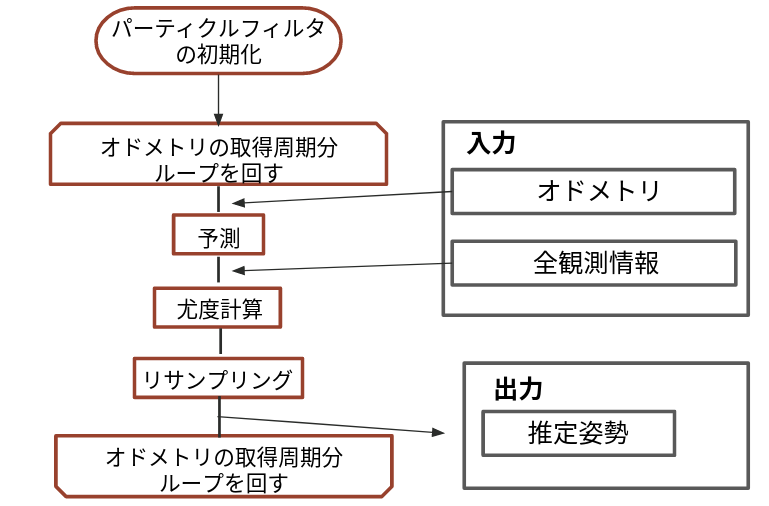
\includegraphics[width=1.2\linewidth]{figs/particle_filter_flow.png}
    \caption{パーティクルフィルタの流れ}
    \label{fig:particle_filter_flow}
  \end{center}
\end{figure}

\chapter{各パーティクルに観測範囲を付与した未知障害物対策}
\section{はじめに}
本章では, 提案手法である, 各パーティクルに観測範囲を付与することで未知障害物の対策をした、
アルゴリズムについて説明する. 
このアルゴリズム[\ref{alg:proposed_mcl}]は、各パーティクルに、自己位置推定に影響を
与えないような観測範囲を与えることによって未知障害物の対応する
アルゴリズムである。
また、従来のパーティクルフィルタに対して、
計算時間の増加なしに、未知障害物による急激な尤度の低下を防ぐことができる。

\begin{figure}[h]
  \begin{algorithm}[H]
      \caption{Proposed MCL($\mathcal{X}_{t-1}, u_t, z_t, m , p_{p\_\mathsf{angle}}$)}
      \label{alg:proposed_mcl}
      \begin{algorithmic}
      \STATE $\mathcal{\bar{X}}_t = \mathcal{X}_t = 0$

      \FOR {$p = 1$ to $P$}
      \STATE $x_{t}^{[p]} = sample\_motion\_model(u_{t}, x_{t-1}^{[p]})$
      \STATE $w_{t}^{[p]} = likelihood\_field\_range\_finder_model\_model(z_{t}, x_{t}^{[p]}, m, p_{p\_\mathsf{angle}})$
      \STATE $\mathcal{\bar{X}}_t = \mathcal{\bar{X}}_t + <x_{t}^{[p]}, w_{t}^{[p]}>$
      \ENDFOR

      \FOR {$p = 1$ to $P$}
      \STATE $draw\;i\;with\;probability \propto w_{t}^{[i]}$
      \STATE $add\; x_{t}^{[i]}\;to\;\mathcal{X}_t$
      \STATE $add\;\;p_{p\_\mathsf{angle}}\;to\;p$
      \STATE $\Uparrow サンプリングしたパーティクルにランダムな観測パターンを付与$
      \ENDFOR
      \FOR {$p = 1$ to $P$}
      \STATE $P_\mathsf{mode\_p\_\mathsf{angle}} \Leftarrow 全パーティクルの中で最瀕な観測パターン$
      \STATE $P_\mathsf{mode\_p\_\mathsf{angle}} = Mode\_p\_\mathsf{angle}(p\rightarrow p_{p\_\mathsf{angle}})$
      \ENDFOR
      
      \RETURN $\mathcal{X}_t, P_\mathsf{mode\_p\_\mathsf{angle}}$
      \end{algorithmic}
  \end{algorithm}
  \caption{提案した手法を用いたMCLの疑似コード}
\end{figure}

\subsection{パーティクルに観測パターンを付与}
まずはじめに、パーティクルフィルタはN個のパーティクルを生成する。
次に、未知障害物を観測した情報を棄却するために図\ref{fig:z_pattern}のような、
観測パターンを用意する。そして、生成された各観測パターンは、N個の各パーティクルに対して
ランダムに与えられる。その後は従来通り、状態遷移モデルに従ってパーティクルをランダムに遷移させる。

\newpage

\begin{figure}[H]
  \begin{center}
    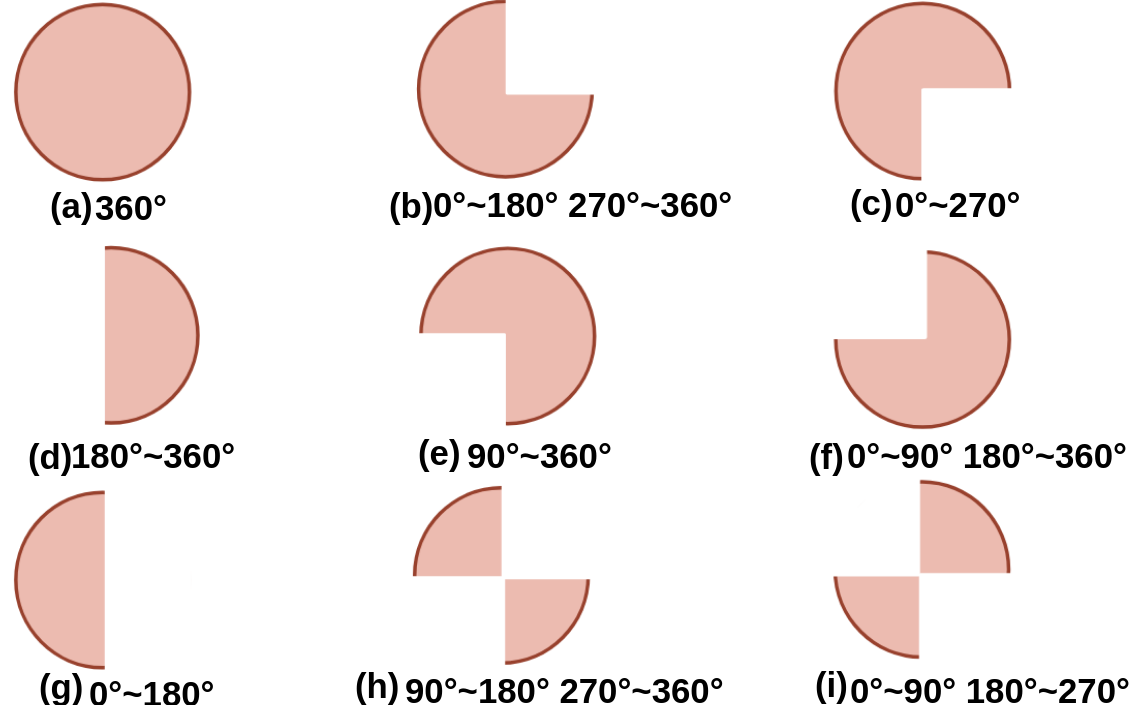
\includegraphics[width=0.8\linewidth]{figs/obs_pangle.png}
    \caption{観測パターン($p_\mathsf{angle}$)}
    \label{fig:1}
  \end{center}
\end{figure}

\subsection{尤度計算による観測パターンの評価}

遷移された各パーティクルの尤もらしさを評価するために尤度場を使用した尤度関数を用いて
各パーティクルの尤度を求める。
観測パターンを持った各パーティクルの尤度は式[\ref{exp:b_p_w_angle}]のように求まる。

\begin{eqnarray}
  \label{exp:b_p_w_angle}
  L_j(x_{t}^{(i)} | z_{j, t}, m, p_\mathsf{angle})
\end{eqnarray}
観測情報$z_t$を観測パターン$p_\mathsf{angle}$によってフィルタをかけることで、使用する観測情報に制限をかけている。
例えば、図\ref{fig:z_pattern}のように、$p_\mathsf{angle} = (a)$を持ったパーティクルであれば、
尤度計算に用いる観測情報は$z_t$の全てである。
$p_\mathsf{angle} = (b)$を持ったパーティクルであれば、尤度計算に用いる観測情報は$360°$のうち$0°〜90°$を間引いた
観測情報$z_t$になる。


\subsection{リサンプリング時にランダムな観測パターンを付与}

パーティクルフィルタの初期化時に、各パーティクルに与えた観測パターンのままであると、
最尤なパーティクルの観測パターンを全てのパーティクル持つことになってしまう。
つまり、ある観測パターンに収束したままになってしまい、環境に応じて
観測パターンを変化させることができない状態に陥る。
そのため、リサンプリング時にN個のパーティクルのうち$\frac{N}{10}$個程度のパーティクルをサンプリングし、
ランダムな観測パターンを与える。

\subsection{尤度計算とリサンプリングによる観測パターンの収束}

以上の尤度計算による観測パターンの評価とリサンプリングによるランダムな観測パターンを持ったパーティクルの
追加によって、パーティクルフィルタは環境に応じて、適した観測パターンを各パーティクルに与えることができる。
そして、全パーティクルで最瀕な観測パターンを求めることで、提案した手法を用いたパーティクルフィルタは、
ロボットの姿勢と環境に適した観測パターンを求めることができる。

\newpage
\section{提案した手法用いたパーティクルフィルタの流れ}

\begin{figure}[h]
  \begin{center}
    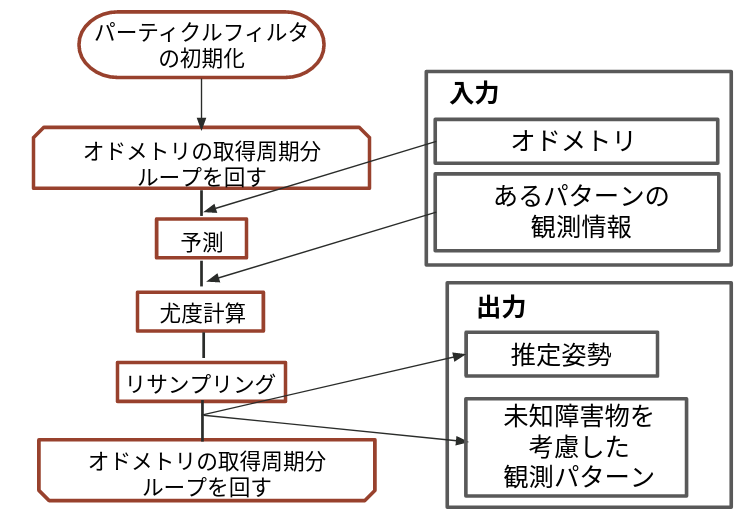
\includegraphics[width=1.0\linewidth]{figs/particle_filter_flow_improve.png}
    \caption{提案した手法用いたパーティクルフィルタの流れ}
    \label{fig:particle_filter_flow_improve}
  \end{center}
\end{figure}

\chapter{シミュレーション実験}\label{chap:simulation_experiment}

\section{はじめに}
本章では, 3章にて提案した手法をMCLに実装し, 
4.5節でシミュレータ環境にて実装した手法による実験結果を示す. 
4.6節にて本章をまとめる. 

\section{環境}

\subsection{シミュレータ環境}

提案したアルゴリズムを評価するために図\ref{fig:sim_world}のような
シミュレータ環境を用いた. 図\ref{fig:sim_world}の環境は図\ref{fig:unknown-obstacles}
の実環境を模したものであり, 図\ref{fig:known-obstacles}の2次元マップを
縦方向に伸ばすことによって作成した3次元の環境である. 
シミュレータ環境内で使用したロボットは, 
Raspberry Pi Cat(以下ラズパイキャット)をモデリングしたものである. 

\subsection{開発環境}
シミュレータの実行および提案手法の実装を行うに当たって, 使用したノートPCの
開発環境を表\ref{tabule:pc_spec_sim}にまとめる. 

\begin{table}[ht]
  \caption{開発環境}
  \label{tabule:pc_spec_sim}
  \begin{center}
    \begin{tabular}{l|c} 
      \thline
      ノートPC& \\
      \hline
      CPU & i7-8665U 1.90GHz \\
      GPU & Quadro P520 \\
      RAM & 32GB  \\
      OS & Ubuntu 18.04 LTS \\
      ROS Distributions & Melodic Morenia \\ 
      \thline
    \end{tabular}
  \end{center}
\end{table}


\begin{figure}[h]
  \begin{center}
    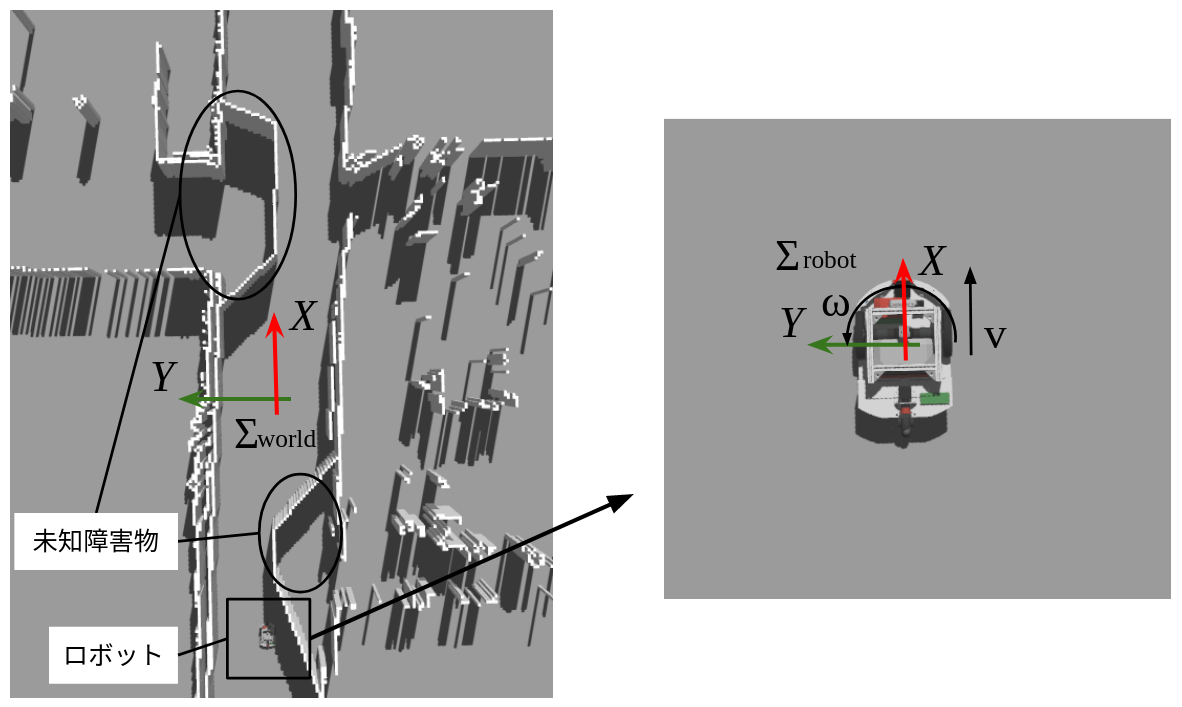
\includegraphics[width=0.98\linewidth]{figs/sim_world.png}
    \caption{使用したシミュレータ環境とロボット}
    \label{fig:sim_world_experiment}
  \end{center}
\end{figure}

\newpage

\begin{figure}[H]
  \begin{center}
    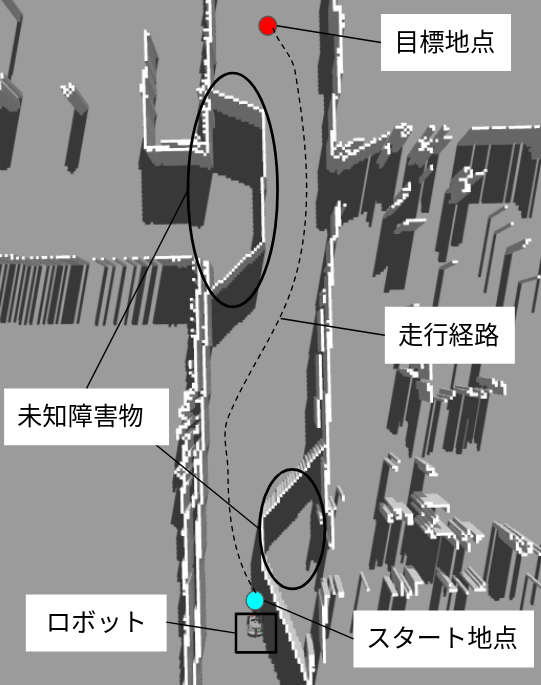
\includegraphics[width=0.5\linewidth]{figs/gazebo_unknown_obstacles.png}
    \caption{スタートと目標地点}
    \label{fig:start_goal_sim}
  \end{center}
\end{figure}

\section{MCLに提案した手法の実装}

提案したアルゴリズムを実装する基になるパッケージとして, 自己位置推定用
のROSパッケージとして公開されているemclを用いる. 
このemclをフォーク[????]して, thesisというブランチで実装を行った. 
実装後のコミット番号はfbb1d9fであり, このコミット番号まで実装した内容について説明していく. 

emclでは, オブジェクト指向を基に, パーティクルフィルタに必要な関数が複数のファイルにて
実装されており, emcl\_node.cpp内でそれらの関数の呼び出しを行っている. 
まず, ExpResetMcl.cppに観測パターンを用意するための関数(generateScanPattern, randomScan)を実装した. 
その関数は, パーティクルの初期化と同時に各パーティクルに対して
図\ref{fig:1}のようなランダムな観測パターンを与える. 
次に, リサンプリング時に, ある観測パターンに収束し続けないように, 全パーティクルのうち$10\%$
のパーティクルをサンプルし, ランダムな観測パターンをそれぞれに与える実装を行った. 

\section{実験方法}

図\ref{fig:sim_world_experiment}のシミュレータ環境用いて, 提案したアルゴリズムを実装したemclの評価を行う. 
実験では未知障害物がある環境を走行した場合において, 以下の項目について評価を行う. 
\begin{itemize}
  \item 走行の評価
  \item 推定された自己位置
  \item 自己位置の尤度
  \item 使用された観測パターン
  \item 尤度計算にかかった時間
\end{itemize}
4.5.1では提案した手法の実装が無い, 4.5.2では提案した手法の実装がある場合において, 
未知障害物が存在するシミュレータ環境で自律走行をした時の評価をまとめる. 

\newpage

\section{実験結果}

\subsection{提案した手法の実装無し}

図\ref{fig:nav_no_imp}のように, 未知障害物が存在するシミュレータ環境において, 提案した手法の実装が無いリセット付きの自己位置推定の場合, 
目標地点にたどり着くことができなかった. これは, 奥側にある未知障害物によって, リセットがかかり続けたため, 
自己位置推定が破綻してしまったことが原因である. 

\begin{figure}[H]
  \begin{center}
    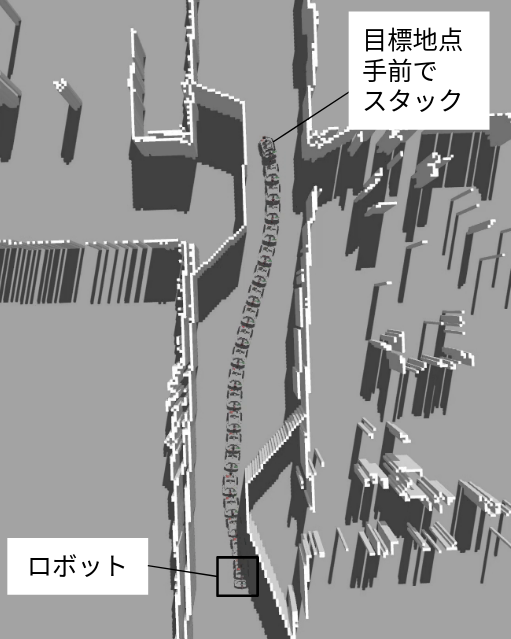
\includegraphics[width=0.5\linewidth]{figs/no_implementation_with_reset.png}
    \caption{未知障害物がある環境での自律走行}
    \label{fig:nav_no_imp}
  \end{center}
\end{figure}

自律走行時のロボットの位置の真値と
走行中に推定された自己位置と比較したグラフは, 図\ref{fig:odom_comp_no_imp}のようになった. 
奥側の未知障害物を走行している20秒辺りでは, 推定された自己位置とロボットの位置の真値として
, x, y方向ともに誤差が生じており, 特にy方向の誤差が大きくなってしまっている. 
これは, 未知障害物によって, 何度もリセットがかかり続けてしまったため, 自己位置推定が不確かになってしまったといえる. 

\begin{figure}[H]
  \begin{center}
    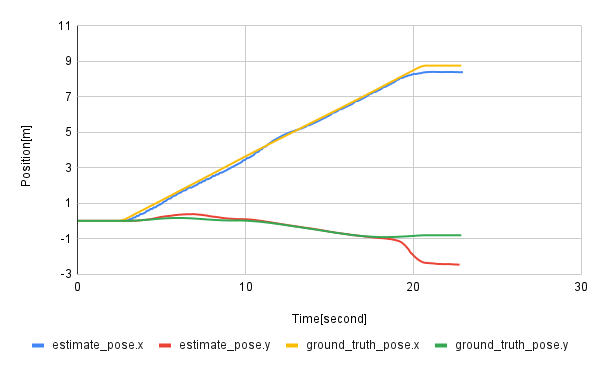
\includegraphics[width=0.98\linewidth]{figs/sim_no_imp_ground_truth.png}
    \caption{推定された自己位置とロボットの位置の真値との比較}
    \label{fig:odom_comp_no_imp}
  \end{center}
\end{figure}

自律走行時の尤度は, 図\ref{fig:nav_likelihood_no_imp}のようになった. 
未知障害物付近を走行している5秒, 20秒辺りでは, ともに尤度が著しく低下してしまっている. 

\begin{figure}[H]
  \begin{center}
    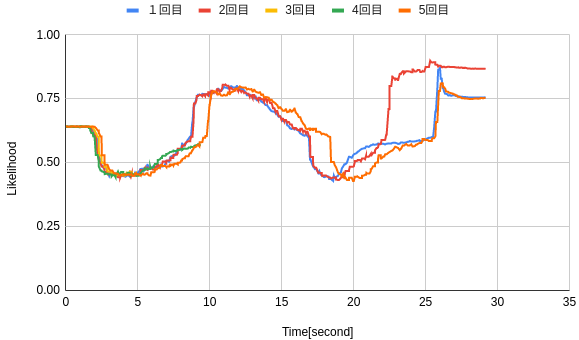
\includegraphics[width=0.98\linewidth]{figs/sim_likelihood_before.png}
    \caption{自律走行時の自己位置の尤度}
    \label{fig:nav_likelihood_no_imp}
  \end{center}
\end{figure}

提案手法の実装が無い場合において, スタートから目標地点までの走行の際に, 
尤度計算にかかった時間は表\ref{tabule:likelihood_calc_time_sim_no_imp}のとおりになった. 

\begin{table}[ht]
  \begin{center}
    \caption{提案手法の実装が無い場合の実験結果}
    \label{tabule:likelihood_calc_time_sim_no_imp}
    \begin{tabular}{l|r|r} 
      \thline
      & 平均[ms] &  標準偏差[ms] \\
      \hline
      尤度計算にかかった時間 & 34.09 & 13.02 \\
      \thline
    \end{tabular}
  \end{center}
\end{table}

\subsection{提案した手法の実装あり}

提案した手法の実装があるリセット付きの自己位置推定では, 目標地点に到達することができた. 

\begin{figure}[H]
  \begin{center}
    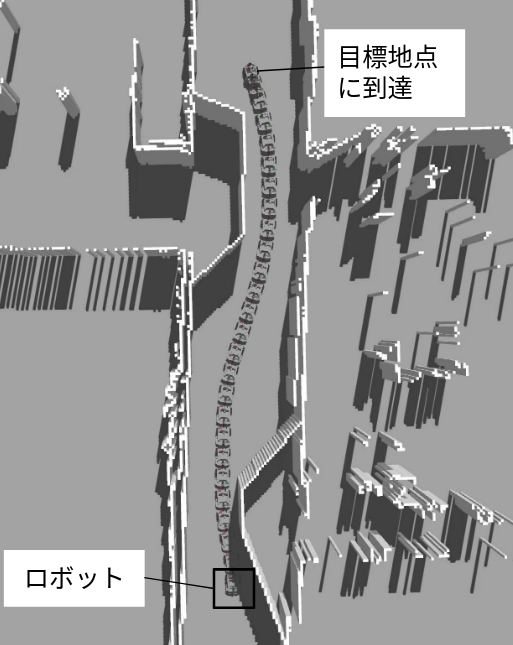
\includegraphics[width=0.5\linewidth]{figs/no_implementation_no_reset.png}
    \caption{未知障害物がある環境での自律走行}
    \label{fig:nav_imp}
  \end{center}
\end{figure}

自律走行時のロボットの位置の真値と
走行中に推定された自己位置と比較したグラフは, 図\ref{fig:odom_comp_imp}のようになった. 
推定された自己位置とロボットの位置の真値を比較して, 目立った誤差はないといえる. 

\begin{figure}[H]
  \begin{center}
    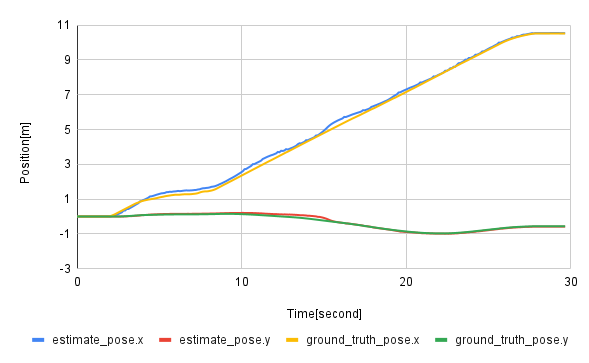
\includegraphics[width=0.98\linewidth]{figs/sim_imp_ground_truth.png}
    \caption{推定された自己位置とロボットの位置の真値との比較}
    \label{fig:odom_comp_imp}
  \end{center}
\end{figure}

自律走行時の尤度は, 図\ref{fig:nav_likelihood_imp}のようになった. 
未知障害物付近の走行時において, 尤度は著しく低下することなく, 安定していることがわかる. 

\begin{figure}[H]
  \begin{center}
    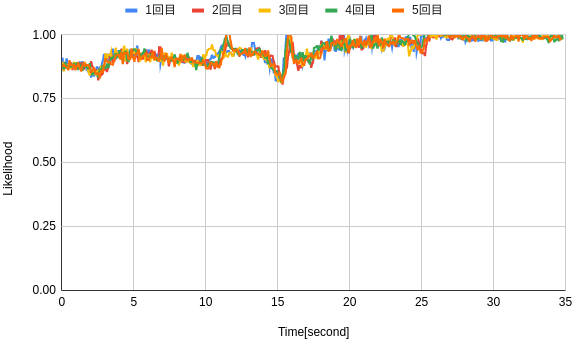
\includegraphics[width=0.98\linewidth]{figs/sim_likelihood_after.png}
    \caption{自律走行時の自己位置の尤度}
    \label{fig:nav_likelihood_imp}
  \end{center}
\end{figure}

自律走行時において, パーティクルの中で最も使用された観測パターンを表したグラフは
図\ref{fig:obs_pattern_sim}のようになった. 
グラフからは, 未知障害物に応じて観測パターンを選択できていることがわかる. 

\begin{figure}[h]
  \begin{center}
    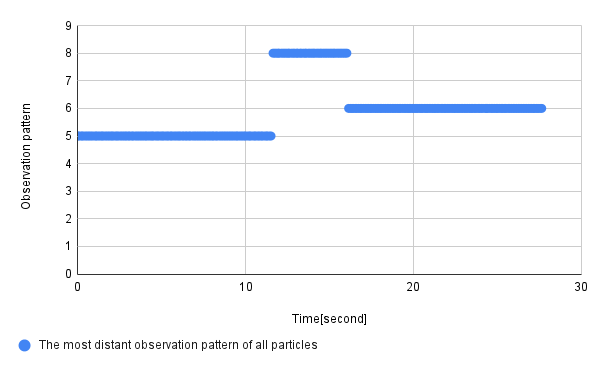
\includegraphics[width=0.98\linewidth]{figs/sim_imp_ob_pattern.png}
    \caption{自律走行時にパーティクルの中で最も使用された観測パターン}
    \label{fig:obs_pattern_sim}
  \end{center}
\end{figure}

提案手法の実装がある場合において, スタートから目標地点までの走行の際に, 
尤度計算にかかった時間は表\ref{tabule:likelihood_calc_time_sim_imp}のとおりになった. 

\begin{table}[ht]
  \begin{center}
    \caption{提案手法の実装がある場合の実験結果}
    \label{tabule:likelihood_calc_time_sim_imp}
    \begin{tabular}{l|r|r} 
      \thline
      & 平均[ms] &  標準偏差[ms] \\
      \hline
      尤度計算にかかった時間 & 30.76 & 6.35 \\
      \thline
    \end{tabular}
  \end{center}
\end{table}

\section{まとめ}
未知障害物が存在するシミュレータ環境において, 提案手法を実装がある場合と無い場合の結果を示した. 
実験の結果から提案手法の実装を行うことで, 未知障害物に影響を受けずに自己位置推定ができることが確認できた. 
また, 提案手法の実装を行うことで, 尤度計算にかかる時間が従来より4[ms]短縮していることも確認できた. 
\chapter{実機実験}\label{chap:practical_experiment}

\chapter{結論}

得られた知見を定量的に述べましょう. 
予稿等では箇条書きにしたほうがよいのですが, 
卒論の場合はどうせ長くなるので箇条書きは不要です. 





\appendix
\chapter*{付録A Raspberry Pi Cat}

\section{Raspberry Pi Cat}
Raspberry Pi Cat(以下ラズパイキャット)は図\ref{fig:raspicat}で示された二輪の差動駆動型ロボットである. 
また, ラズパイキャットは既製品の小型移動ロボットである.
このロボットについて説明をする.
\begin{figure}[h]
	\begin{center}
		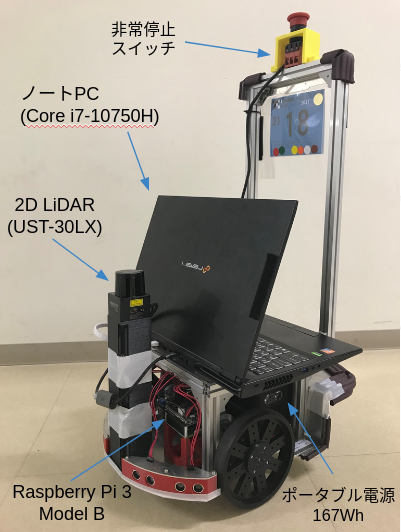
\includegraphics[width=0.5\linewidth]{figs/raspicat.png}
		\caption{}
		\label{fig:raspicat}
	\end{center}
\end{figure}

\subsection{使用したコンピュータのスペック}

\subsubsection{Raspberry Pi 3 Model B}
SoCはBroadcom BCM2837 1.2GHz×4(CPU).
メモリは1GB.
\subsubsection{ノートPC}
CPUはCore i7-10750H 2.6GHz×12. 
GPUはNVIDIA GeForce RTX 2070.
メモリは32GB.

\subsection{2D LiDAR}
使用した2D LiDARはHOKUYOのUST-30LXである.
UST-30LXの走査角度は270度, 角度分解能は0.25度, 測定分解能は1mm, 最大検出距離は60mである.

地面などのノイズを観測せずに多くのランドマークを獲得するために図\ref{fig:raspicat-lidar}
のように地面から36cmの高さに取り付けた.

\begin{figure}[h]
	\begin{center}
		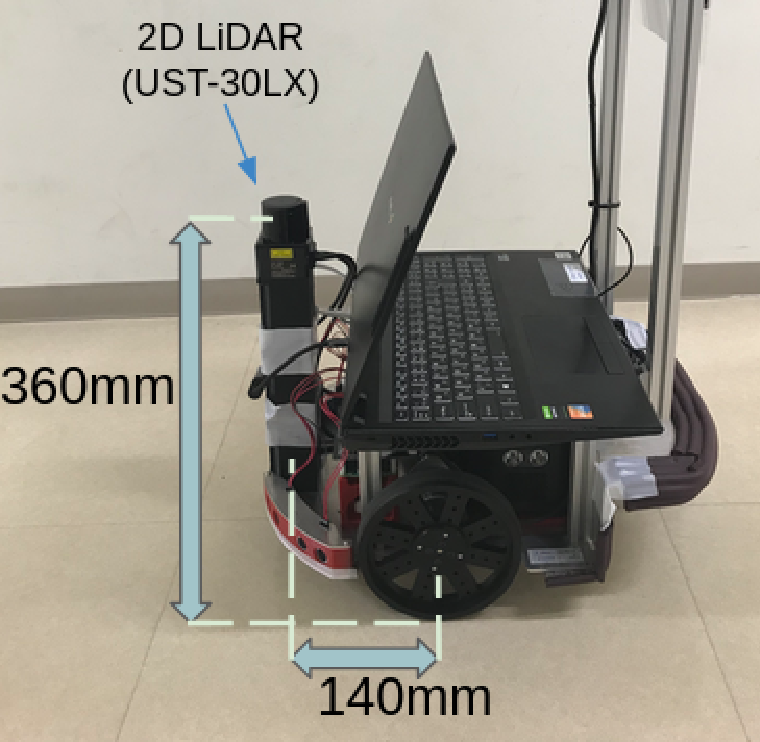
\includegraphics[width=0.5\linewidth]{figs/raspicat-lidar.pdf}
		\caption{}
		\label{fig:raspicat-lidar}
	\end{center}
\end{figure}

\subsection{ハードウェア構成}
ラズパイキャットのハードウェア構成を図\ref{fig:raspicat-hardware-config}に示す. 
搭載されている外界センサは, 2D LiDAR(UST-30LX)のみである.この2D LiDARのみで
自己位置推定や障害物回避を実現している. 
モータの速度制御としてRaspberry Pi 3 Model Bが搭載されており, モータは
Raspberry Pi 3 Model Bから送られてくる速度指令値に基づいてモータドライバによって駆動されている.

自己位置推定や行動計画のための計算機としてノートPC(Intel i7-10750H)を搭載している.
また, Raspberry Pi 3 Model BとノートPCはLANケーブルによる接続で通信を行っている.

\begin{figure}[h]
	\begin{center}
		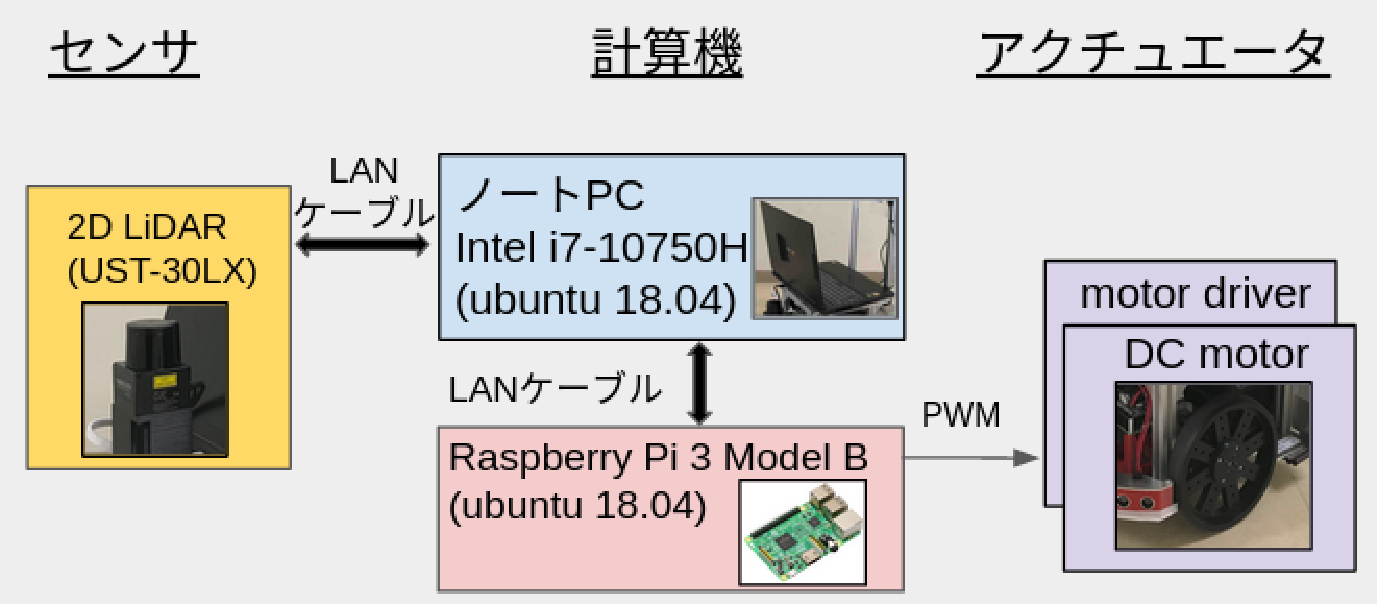
\includegraphics[width=1.0\linewidth]{figs/raspicat-hardware-config.pdf}
		\caption{}
		\label{fig:raspicat-hardware-config}
	\end{center}
\end{figure}

\subsection{ソフトウェア構成}
ラズパイキャットのソフトウェア構成を図\ref{fig:raspicat-software-config}に示す.
ラズパイキャットはロボットの制御システムとしてROSを使用している.Raspberry Pi 3 Model Bではmotorsノードのみが立ち上がっており, 
モータの制御を行っている. 
ノートPCでは, amclやmove\_base等のノードが立ち上がっており, 
自己位置推定や行動計画を行っている.

オドメトリにはimuなどは使用しておらず, 
motorsノードで速度指令値(/cmd\_vel)を積算させたデッドレコニング(/odom)を使用している. 
そのため, 急回転には弱いが非常に簡素なシステムになっているためシステムの
立ち上げミスが少ない.



\begin{figure}[H]
	\begin{center}
		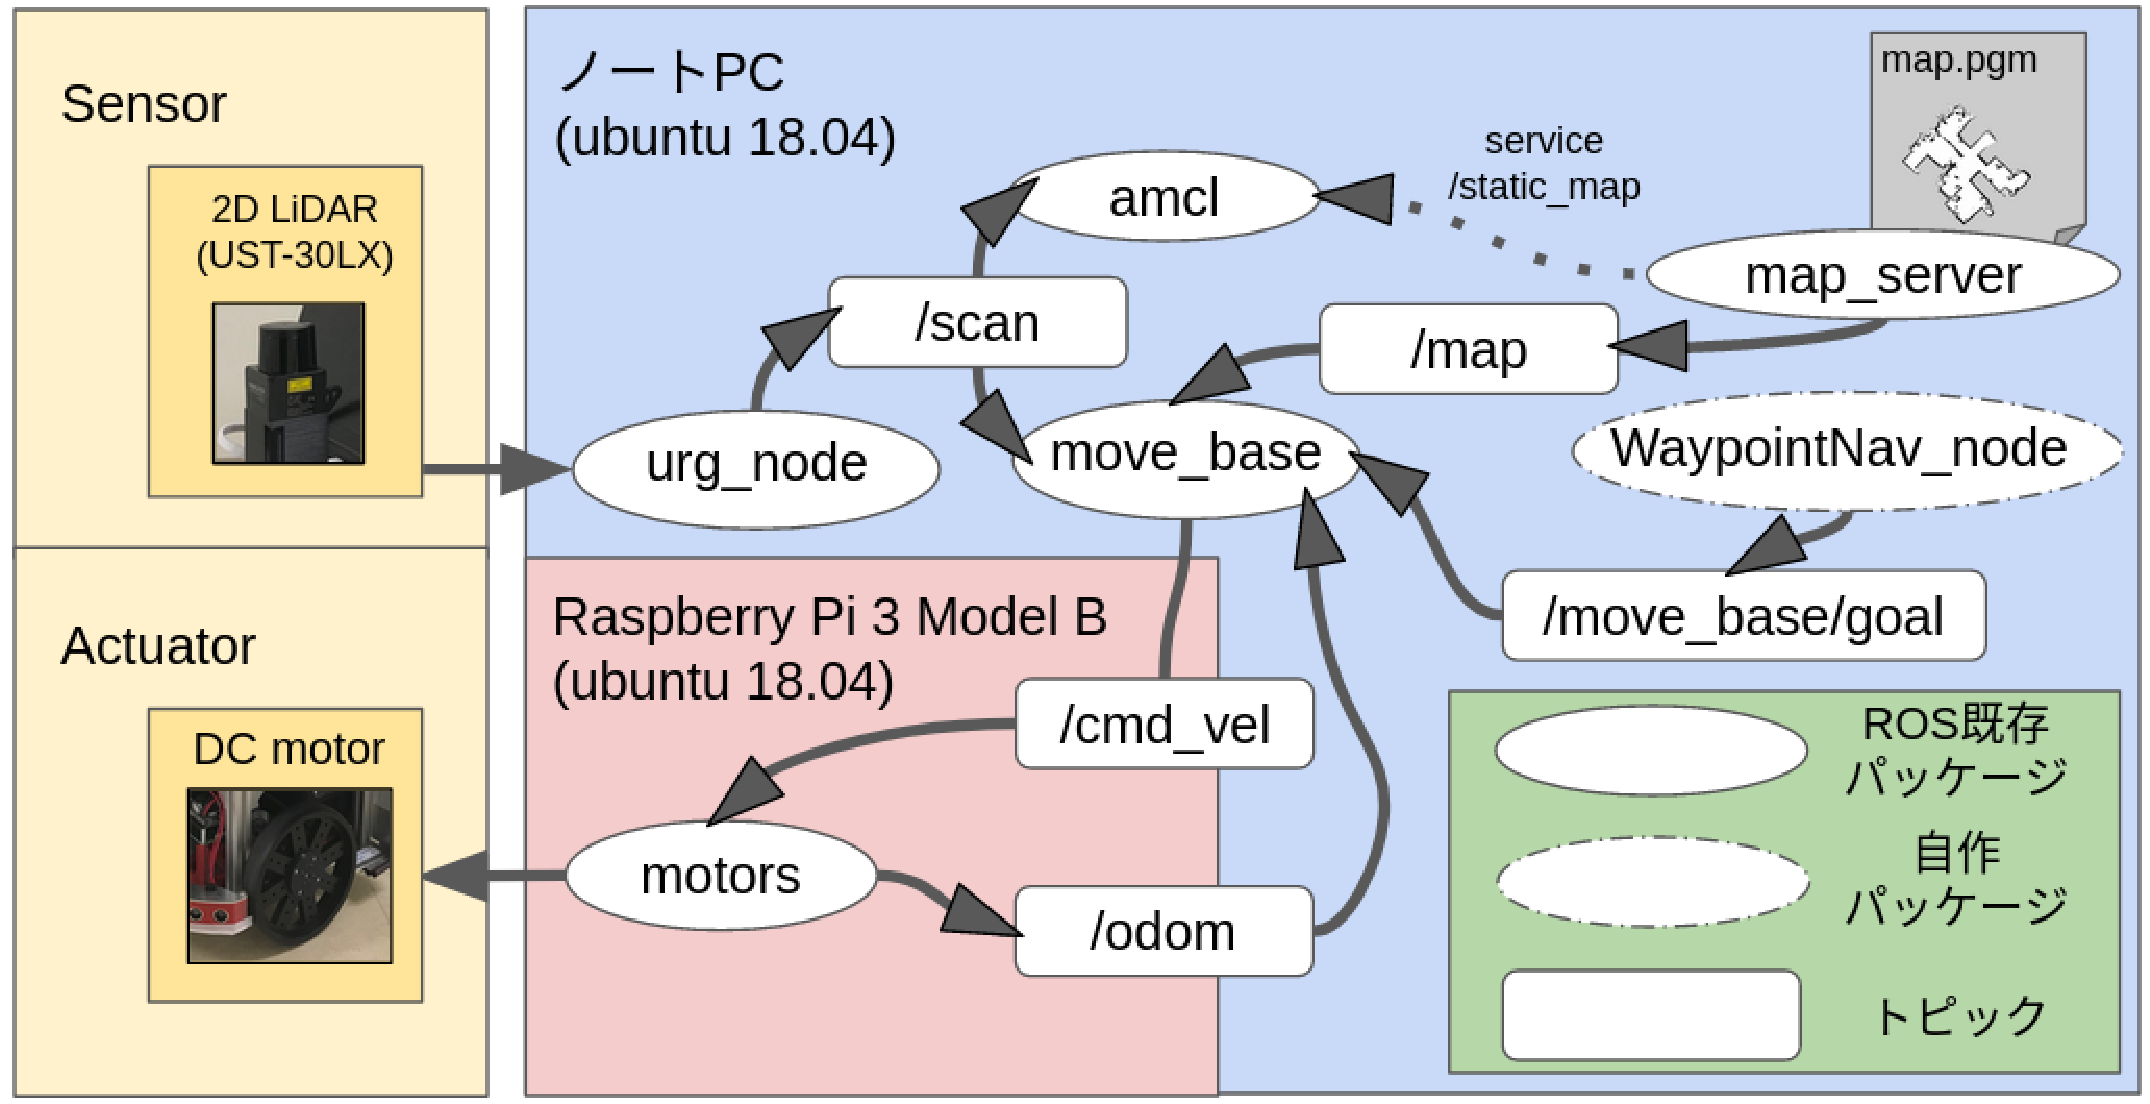
\includegraphics[width=0.9\linewidth]{figs/raspicat-software-config.pdf}
		\caption{}
		\label{fig:raspicat-software-config}
	\end{center}
\end{figure}

% %% 参考文献 %%%
% よほどのことが無い限りet al.は使わないことにしましょう
% \bibliographystyle{unsrt}
% \bibliography{./references}

\begin{thebibliography}{99}

  \bibitem{mcl}
    Jens-Steffen Gutmann and Dieter Fox: An Experimental Comparison of Localization Methods Continued, 
    Princeton University Press(1957), Proc. of the \textit{IROS}, pages 454-459, 2002.
  \bibitem{amcl}
    ROS.org:``amcl'', \url{https://wiki.ros.org/amcl} (last visit: 2021-10-20).
  \bibitem{emcl}
    Ryuichi Ueda: ``ryuichiueda/emcl'', \url{https://github.com/ryuichiueda/emcl} (last visit: 2021-10-20). 
  \bibitem{ueda2004iros}
    Ryuichi Ueda and Tamio Arai and Kohei Sakamoto and Toshifumi Kikuchi and Shogo Kamiya: 
    ``Expansion Resetting for Recovery from Fatal Error in Monte Carlo Localization -- Comparison with Sensor Resetting Methods,'' Proc. of IROS, pp.2481--2486, 2004.  
  \bibitem{富沢}
    冨沢 哲雄 and 村松 聡 and 平井 雅尊 and 佐藤 晶則 and 工藤 俊亮 and 末廣 尚士:
    ``グリッドマップのマッチングに基づく未知障害物にロバストな自己位置推定'', 日本ロボット学会誌, 30(3):280-286, 2012.
  \bibitem{赤井}
    赤井 直紀 and モラレス ルイス 洋一 and 平山 高嗣 and 村瀬 洋:
    ``幾何地図上での観測物体の有無を考慮した自己位置推定'', 計測自動制御学会論文集, 55(11):745-753, 2019.
  \bibitem{raspicat}
    ROS.org:``ja/raspicat'', \url{https://wiki.ros.org/ja/raspicat} (last visit: 2021-10-20). 
  \bibitem{RTshop}
    株式会社アールティ:``Raspberry Pi Cat 屋外でも動かせる中型2輪ロボット'', 
    RT Robot Shop Products, \url{https://rt-net.jp/products/raspberry-pi-cat/}(last visit 2021-10-16)
  \bibitem{UST-30LX}
    株式会社北陽:``UST-30LX'', 
    製品概要, \url{https://www.hokuyo-aut.co.jp/search/single.php?serial=195#spec}(last visit 2022-2-24)
  \end{thebibliography}

\newpage
\printindex

\end{document}


